\documentclass[10pt,a4paper]{article}
\usepackage[utf8x]{inputenc}
\usepackage{ucs}
\usepackage{amsmath}
\usepackage{amsfonts}
\usepackage{amssymb}
\usepackage{graphicx}

\usepackage{tikz}

\begin{document}
    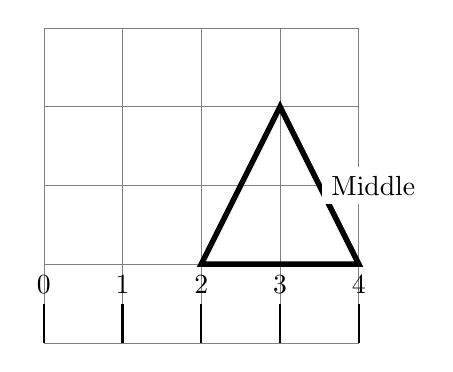
\begin{tikzpicture}
    
    % \clip (0.5,0.5) rectangle (3.5,3.5);
    \draw[help lines] (0,0) grid (4,4);
    
    \begin{scope}[line width=2]
    \draw[xshift=1cm]
    (1,1) to
    (3,1) to node[anchor=west,fill=white] {Middle}
    (2,3) to
    cycle;
    \end{scope}
    
    \foreach \x in {0,1,...,4} {
        \draw[thick] (\x,0) to (\x,.5) node[anchor=south] {\x};
    }
    
    \end{tikzpicture}
\end{document}